\documentclass[11pt,a4paper]{report}
\usepackage[margin=1in]{geometry}
\usepackage{xcolor}
\usepackage[sf,bf]{titlesec}
\usepackage{graphicx}
\usepackage{amsmath}
\usepackage{amsthm}
\usepackage{amsfonts,amssymb}
\usepackage{mathtools}
\usepackage{framed}
\usepackage{mdframed}
\usepackage[style=trad-abbrv,doi=true,url=true,isbn=false,backend=bibtex]{biblatex}
\usepackage{setspace}
\usepackage{algpseudocode}
\usepackage{algorithm}
\usepackage{fontawesome}
\usepackage{hyperref}
\usepackage[nameinlink,capitalise]{cleveref}
\usepackage{multicol}
\usepackage{tikz-cd}

% \setlength{\parskip}{4pt}
\onehalfspacing

\usepackage{pgfplots}
\pgfplotsset{compat=1.16}
\usetikzlibrary{graphs,graphdrawing}
\usetikzlibrary{backgrounds}
\usegdlibrary{trees}
\usegdlibrary{force}

% Code listings
\usepackage[cache=true,outputdir=build]{minted}
\usepackage{caption}
\newenvironment{code}{\captionsetup{type=listing}}{}
% \SetupFloatingEnvironment{listing}{name=Listing}

% Colors
\definecolor{lightblue}{HTML}{f1f8fb}
\definecolor{lightgreen}{HTML}{f1faf8}
\definecolor{darkblue}{HTML}{315a88}
\definecolor{lightred}{HTML}{f8f6ee}
\definecolor{lightcyan}{rgb}{0.84,1,1}
\definecolor{lightred}{rgb}{1,0.7,0.71}
\definecolor{nicegreen}{rgb}{0.64,1,0.71}

\hypersetup{%
    linktocpage=true,
    colorlinks=true,
    urlcolor=darkblue,
    linkcolor=darkblue,
    citecolor=darkblue,
    pdfauthor={Urbain Vaes}
    pdftitle={Lecture notes in Numerical Analysis}
    pdfsubject={Applied mathematics}
}

% Define frames
\newenvironment{myframe}
{%
    \begin{mdframed}[
        leftmargin=0cm,
        skipabove=.3cm,
        linecolor=blue,
        backgroundcolor=lightblue,
        linewidth=0pt,
        innerleftmargin=.5em,
        innerrightmargin=.5em,
        innertopmargin=.3em,
        innerbottommargin=.6em,
    ]
}
{
    \end{mdframed}
}

\newenvironment{solutionframe}
{%
    \begin{mdframed}[
        leftmargin=1cm,
        skipabove=.3cm,
        linecolor=blue,
        backgroundcolor=lightgreen,
        linewidth=0pt,
        innerleftmargin=.5em,
        innerrightmargin=.5em,
        innertopmargin=.3em,
        innerbottommargin=.6em,
    ]
}
{
    \end{mdframed}
}

% Fonts for lualatex
\usepackage{fontspec}
% \setmonofont{Monaco}[Scale=MatchLowercase,BoldFont=DejaVu sans Mono-bold]
% \setmonofont{DejaVu sans Mono}[Scale=MatchLowercase,BoldFont=DejaVu sans Mono-bold]
\setmonofont{Latin Modern Mono}[%
    Scale=MatchLowercase,
    ItalicFont=Latin Modern Mono,
    BoldItalicFont=DejaVu sans Mono-bold,
    BoldFont=DejaVu sans Mono-bold]
% \setmainfont{DejaVu Serif}
\usepackage{newunicodechar}
% To check that a font supports Greek letters, try 'albatross α'
\newfontfamily{\fallbackfont}{DejaVu Sans Mono}[Scale=MatchLowercase]
\DeclareTextFontCommand{\textfallback}{\fallbackfont}
\newunicodechar{α}{\textfallback{α}}
\newunicodechar{β}{\textfallback{β}}
\newunicodechar{γ}{\textfallback{γ}}
\newunicodechar{δ}{\textfallback{δ}}
\newunicodechar{ε}{\textfallback{ε}}
\newunicodechar{ζ}{\textfallback{ζ}}
\newunicodechar{η}{\textfallback{η}}
\newunicodechar{θ}{\textfallback{θ}}
\newunicodechar{ι}{\textfallback{ι}}
\newunicodechar{κ}{\textfallback{κ}}
\newunicodechar{λ}{\textfallback{λ}}
\newunicodechar{μ}{\textfallback{μ}}
\newunicodechar{ν}{\textfallback{ν}}
\newunicodechar{ξ}{\textfallback{ξ}}
\newunicodechar{ο}{\textfallback{ο}}
\newunicodechar{π}{\textfallback{π}}
\newunicodechar{ρ}{\textfallback{ρ}}
\newunicodechar{σ}{\textfallback{σ}}
\newunicodechar{τ}{\textfallback{τ}}
\newunicodechar{υ}{\textfallback{υ}}
\newunicodechar{φ}{\textfallback{φ}}
\newunicodechar{χ}{\textfallback{χ}}
\newunicodechar{ψ}{\textfallback{ψ}}
\newunicodechar{ω}{\textfallback{ω}}
\newunicodechar{Α}{\textfallback{Α}}
\newunicodechar{Β}{\textfallback{Β}}
\newunicodechar{Γ}{\textfallback{Γ}}
\newunicodechar{Δ}{\textfallback{Δ}}
\newunicodechar{Ε}{\textfallback{Ε}}
\newunicodechar{Ζ}{\textfallback{Ζ}}
\newunicodechar{Η}{\textfallback{Η}}
\newunicodechar{Θ}{\textfallback{Θ}}
\newunicodechar{Ι}{\textfallback{Ι}}
\newunicodechar{Κ}{\textfallback{Κ}}
\newunicodechar{Λ}{\textfallback{Λ}}
\newunicodechar{Μ}{\textfallback{Μ}}
\newunicodechar{Ν}{\textfallback{Ν}}
\newunicodechar{Ξ}{\textfallback{Ξ}}
\newunicodechar{Ο}{\textfallback{Ο}}
\newunicodechar{Π}{\textfallback{Π}}
\newunicodechar{Ρ}{\textfallback{Ρ}}
\newunicodechar{Σ}{\textfallback{Σ}}
\newunicodechar{Τ}{\textfallback{Τ}}
\newunicodechar{Υ}{\textfallback{Υ}}
\newunicodechar{Φ}{\textfallback{Φ}}
\newunicodechar{Χ}{\textfallback{Χ}}
\newunicodechar{Ψ}{\textfallback{Ψ}}
\newunicodechar{Ω}{\textfallback{Ω}}

% Style of sections (sectsty)
% \usepackage{sectsty}
% \allsectionsfont{\sffamily}
% \sectionfont{\sffamily\color{darkblue}}

% Style of sections (titlesec)
\makeatletter
\newcommand*\@secondofsix[6]{#2}
\newcommand{\addtotitleformat}{%
  \@ifstar{\addtotitleformat@star}{\addtotitleformat@nostar}}
\newcommand\addtotitleformat@nostar[2]{%
  \PackageError{titlesec}{non starred form of \string\addtotitleformat\space not supported}{}}
\newcommand\addtotitleformat@star[2]{%
  \expandafter\expandafter\expandafter\expandafter
  \expandafter\expandafter\expandafter\def
  \expandafter\expandafter\expandafter\expandafter
  \expandafter\expandafter\expandafter\@currentsection@font
  \expandafter\expandafter\expandafter\expandafter
  \expandafter\expandafter\expandafter{%
    \expandafter\expandafter\expandafter\@secondofsix
       \csname ttlf@\expandafter\@gobble\string#1\endcsname}%
  \titleformat*{#1}{\@currentsection@font#2}}
\makeatother
\addtotitleformat*{\section}{\color{darkblue}}

% Numbering of equations
\numberwithin{equation}{chapter}

% Equations and theorems
\theoremstyle{plain}% default
\newtheorem{prototheorem}{Theorem}[chapter]
\newtheorem{protoproposition}[prototheorem]{Proposition}
\newtheorem{protolemma}[prototheorem]{Lemma}
\newtheorem{protocorollary}[prototheorem]{Corollary}
\newtheorem{protoexercise}{{\normalfont \faGears}~Exercise}[chapter]
\newtheorem{protocompexercise}[protoexercise]{{\normalfont \faLaptop}~Exercise}
\newtheorem{task}{{\normalfont \faLaptop}~Task}
\theoremstyle{definition}
\newtheorem{protodefinition}{Definition}[chapter]
\newtheorem{protonotation}{Notation}[chapter]
\theoremstyle{remark}
\newtheorem{protoexample}{Example}[chapter]
\newtheorem{protoremark}{Remark}[chapter]
\newtheorem*{protosolution}{Solution}

\newenvironment{solution}
{\pushQED{\qed}\renewcommand{\qedsymbol}{$\triangle$}
\begin{solutionframe}\small \begin{protosolution}}
{\popQED\end{protosolution}\end{solutionframe}}

% Minitoc
\usepackage[nohints]{minitoc}
\setcounter{tocdepth}{1}
\setcounter{minitocdepth}{2}
\renewcommand{\mtctitle}{}
\nomtcrule

% Styling of Theorems
\colorlet{theoremcolor}{lightblue}
\colorlet{propositioncolor}{lightblue}
\colorlet{lemmacolor}{lightblue}
\colorlet{corollarycolor}{lightblue}
\colorlet{examplecolor}{lightblue}
\colorlet{definitioncolor}{lightblue}
\colorlet{notationcolor}{lightblue}
\colorlet{remarkcolor}{lightblue}
\newenvironment{theorem}
   {\colorlet{shadecolor}{theoremcolor}\begin{shaded}\begin{prototheorem}}
   {\end{prototheorem}\end{shaded}}
\newenvironment{proposition}
   {\colorlet{shadecolor}{propositioncolor}\begin{myframe}\begin{protoproposition}}
   {\end{protoproposition}\end{myframe}}
\newenvironment{lemma}
   {\colorlet{shadecolor}{lemmacolor}\begin{shaded}\begin{protolemma}}
   {\end{protolemma}\end{shaded}}
\newenvironment{corollary}
   {\colorlet{shadecolor}{corollarycolor}\begin{shaded}\begin{protocorollary}}
   {\end{protocorollary}\end{shaded}}
\newenvironment{example}
   {\colorlet{shadecolor}{examplecolor}\begin{shaded}\begin{protoexample}}
   {\end{protoexample}\end{shaded}}
\newenvironment{definition}
   {\colorlet{shadecolor}{definitioncolor}\begin{myframe}\begin{protodefinition}}
   {\end{protodefinition}\end{myframe}}
\newenvironment{notation}
   {\colorlet{shadecolor}{notationcolor}\begin{shaded}\begin{protonotation}}
   {\end{protonotation}\end{shaded}}
\newenvironment{remark}
   {\colorlet{shadecolor}{remarkcolor}\begin{myframe}\begin{protoremark}}
   {\end{protoremark}\end{myframe}}
\newenvironment{exercise}
   {\colorlet{shadecolor}{white}\begin{protoexercise}}
   {\end{protoexercise}}
\newenvironment{compexercise}
   {\colorlet{shadecolor}{white}\begin{protocompexercise}}
   {\end{protocompexercise}}

% Links
\crefname{protolemma}{Lemma}{Lemmas}
\crefname{prototheorem}{Theorem}{Theorems}
\crefname{protoproposition}{Proposition}{Propositions}
\crefname{protocorollary}{Corollary}{Corollarys}
\crefname{protoexample}{Example}{Examples}
\crefname{protodefinition}{Definition}{Definitions}
\crefname{protoremark}{Remark}{Remarks}
\crefname{protoexercise}{Exercise}{Exercises}
\crefname{protocompexercise}{Exercise}{Exercises}
\crefname{code}{Julia listing}{Julia listings}
\crefname{figure}{Figure}{Figures}
% \Crefname{algorithm}{Algorithm}{Algorithms}

% Bibliography
\addbibresource{references.bib}
\renewcommand*{\mkbibnamegiven}[1]{\textsc{#1}}
\renewcommand*{\mkbibnamefamily}[1]{\textsc{#1}}
\DeclareFieldFormat{volume}{volume \textbf{#1}}
\DeclareFieldFormat[article]{volume}{\textbf{#1}}
\DeclareFieldFormat[book]{note}{}
\DeclareFieldFormat[book]{pages}{}
\DeclareFieldFormat{url}{\newline {\scriptsize\textsc{url}: \url{#1}}}
\DeclareFieldFormat{doi}{\newline {\scriptsize\textsc{doi}: \url{#1}}}
\renewcommand*{\bibfont}{\small}

% Custom cite command
\DeclareCiteCommand{\fullcite}
  {\usebibmacro{prenote}}
  {\clearfield{doi}%
   \clearfield{pages}%
   \clearfield{pagetotal}%
   \clearfield{edition}%
   \clearfield{labelyear}%
   \usedriver
     {\DeclareNameAlias{sortname}{default}}
     {\thefield{entrytype}}}
  {\multicitedelim}
  {\usebibmacro{postnote}}

% Headers
\usepackage{fancyhdr}
\usepackage{emptypage}

% Clear defaults
\fancyhead{}

% Left-Odd, Right-Even
\definecolor{darkgrey}{RGB}{120,120,120}
% \fancyhead[LE,RO]{\color{darkgrey}\textit{\nouppercase{\leftmark}}}
\fancyhead[R]{\color{darkgrey}\textit{\nouppercase{\leftmark}}}
% \fancyhead[LO,RE]{\color{darkgrey}\textit{\thepage}}
% \fancyhead[LO,RE]{}
% \fancyfoot[C]{\color{darkgrey}\textit{\thepage}}
\fancyfoot[C]{\thepage}
\pagestyle{fancy}
\let\oldheadrule\headrule
\renewcommand{\headrule}{}
% \renewcommand{\headrule}{\color{darkgrey}\oldheadrule}
% \renewcommand{\headrulewidth}{0pt}
\setlength{\headheight}{13.59999pt}

\setlength{\OuterFrameSep}{0pt}

\DeclarePairedDelimiter\abs{\lvert}{\rvert}
\DeclarePairedDelimiter\norm{\lVert}{\rVert}
\DeclarePairedDelimiter\ip{\langle}{\rangle}

\DeclareMathOperator{\diag}{diag}
\DeclareMathOperator{\cond}{cond}
\DeclareMathOperator{\Span}{span}
\DeclareMathOperator{\sign}{sign}
\DeclareMathOperator{\spectrum}{spectrum}
\DeclareMathOperator*{\trace}{tr}
\DeclareMathOperator*{\argmin}{arg\,min}
\DeclareMathOperator*{\argmax}{arg\,max}

\renewcommand{\d}{\mathrm d}
\renewcommand{\t}{T}
\newcommand{\e}{\mathrm e}
\newcommand{\D}{\mathrm D}
\newcommand{\real}{\mathbf R}
\newcommand{\poly}{\mathbf P}
\newcommand{\complex}{\mathbf C}
\newcommand{\nat}{\mathbf N}
\newcommand{\integer}{\mathbf Z}
\newcommand{\floating}{\mathbf F}
\newcommand{\madd}{\mathbin{\widehat +}}
\newcommand{\mtimes}{\mathbin{\widehat *}}
\newcommand{\msub}{\mathbin{\widehat -}}
\newcommand{\vect}[1]{\mathbf{\boldsymbol{#1}}}
\newcommand{\mat}{\mathsf}
\newcommand{\placeholder}{\mathord{\color{black!33}\bullet}}%
\newcommand{\moreinfo}{\texorpdfstring{{\normalfont \color{lightred}$^{\text{\faSearchPlus}}$}}{}}
\newcommand{\laplacian}{\triangle}
\newcommand{\julia}[1]{\mintinline{julia}{#1}}


\title{\vspace{-1cm}\textbf{Numerical Analysis} \\[1cm]
    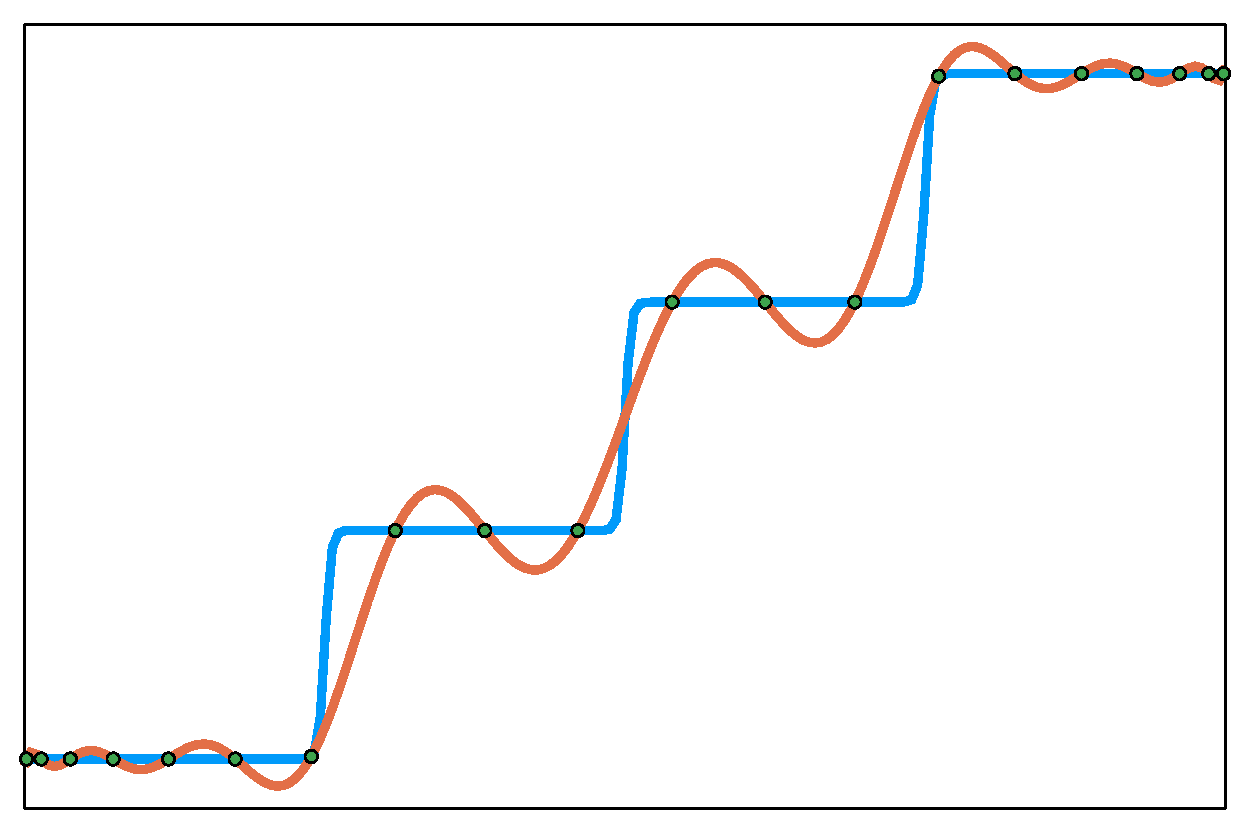
\includegraphics[width=.7\textwidth]{figures/chebychev_cover.pdf}
    % 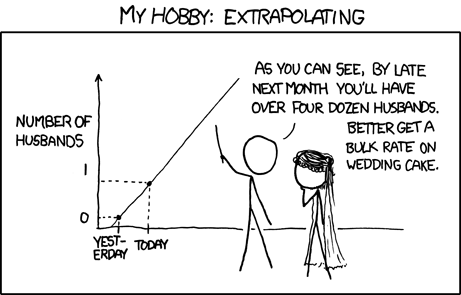
\includegraphics[width=.7\textwidth]{figures/extrapolating.png}
}
\author{%
    Urbain \textsc{Vaes} \\
    \texttt{urbain.vaes@inria.fr}
}
\date{\vspace{1cm} {\large\textsc{NYU Paris}, Spring term 2022} \\[2cm]
    \vfill
    \flushleft \textbf{Weekly schedule}:
    \begin{itemize}
        \item Lectures on Tuesday and Thursday afternoon (2 $\times$ 1h15);
        \item Recitation on Thursday afternoon (1h30);
        \item Office hour on Tuesday, after the lecture.
    \end{itemize}
}
\begin{document}
\maketitle

\chapter*{License}%
\label{cha:license}

The copyright of these notes rests with the author and
their contents are made available under a Creative Commons
\href{https://creativecommons.org/licenses/by-sa/4.0/}{``Attribution-ShareAlike 4.0 Interational''}
license.
You are free to copy, distribute, transform and build upon the thesis under the following terms:
\begin{itemize}
    \item \textbf{Attribution.}
    You must give appropriate credit, provide a link to the license, and indicate if changes were made.
    You may do so in any reasonable manner, but not in any way that suggests the licensor endorses you or your use.
    \item \textbf{ShareAlike.} If you remix, transform, or build upon the material,
        you must distribute your contributions under the same license as the original.
\end{itemize}

\vspace{1cm}
\hfill 
\includegraphics[scale=.7]{figures/cc-by-sa.pdf}

\chapter*{Introduction}%
In a wide variety of scientific disciplines,
ranging from physics to biology and economics,
the phenomena under consideration are well-described by mathematical equations.
More often than not,
these equations are too difficult to be solved analytically,
and so one has to recur to \emph{computer calculations} in order to obtain approximate solutions.
Practical applications in which computer simulation plays a crucial role include
weather forecasting, drug discovery through molecular modeling,
flight simulation, and structural engineering, to mention just a few.

% Since computers have finite memory,
% they are not able to store
% continuous mathematical objects,
% such as solutions to partial differential equations, are represented using finite arrays of numbers,
% which introduces an approximation error.
% When approximating
% It is important to understand the error induced by the use of numerical simulation,
% As application domains where computer simulation is particularly important,
% we mention weather forecasting

Numerical simulation may also be employed in order to calibrate mathematical models of physical phenomena,
particularly when observation through experiment is impractical or too costly.
For example, it is frequently the case that the parameters in mathematical models for turbulence are estimated not from real data,
but from synthetic data generated by computer simulation of the fundamental equations of fluid mechanics.
Relying on ``computer experiments'' is attractive in this context because
these enable to perform accurate measurements without disturbing the system being observed.
Numerical simulation is also very useful to understand and build simplified models for physical phenomena at very small scales,
where direct observation is beyond the current capabilities of experimental physics.

The aim of this course is to present the standard numerical methods for performing the tasks most commonly encountered in applications:
the solution of linear and nonlinear systems of equations,
the solution of eigenvalue problems,
interpolation and approximation of functions,
and numerical integration.
For a given task,
there are usually many numerical methods to choose from,
and these often include parameters which must be fixed appropriately in order to guarantee a good efficiency.
In order to understand what method to employ for best results according to the context,
we study carefully the \emph{convergence properties} of the methods considered.
Six topics will be covered in these lecture notes.
\begin{itemize}
    \item
        \textbf{Floating point arithmetic.}
        In~\cref{cha:rounding_errors},
        we discuss how real numbers are represented, manipulated and stored on a computer.
        There is an uncountable infinity of real number,
        but only a finite subset of these can be represented exactly on a computer.
        This subset is specified in the~\emph{IEEE 754} standard,
        which is widely accepted today and employed in most programming languages, including \texttt{Julia}.

    \item
        \textbf{Solution of linear systems.}
        In \cref{cha:solution_of_linear_systems},
        we study the most widely-used numerical methods for solving linear systems.
        Linear systems are ubiquitous in science,
        often arising from the discretization of linear elliptic partial differential equations,
        which themselves govern a large number of physical phenomena including heat propagation, electromagnetism, gravitation and the deformation of solids.
        % using for example a finite difference method.
        A subclass of linear systems, in which the matrix on the left-hand side is positive semi-definite,
        also appear in the context of optimization:
        indeed, if $A \in \real^{n \times n}$ is positive definite and $b \in \real^n$,
        then the unique minimizer of $\frac{1}{2} x^\t A x - b^\t x$ satisfies the linear system $A x = b$.

    \item
        \textbf{Solution of nonlinear equations.}
        In \cref{cha:solution_of_nonlinear_systems},
        we present widely-used methods for solving nonlinear equations.
        Like linear equations, nonlinear equations are omnipresent in science,
        a prime example being the Navier--Stokes equation describing the motion of fluid flows.
        They are usually much more difficult to solve and require dedicated techniques.
        In addition, the solution to nonlinear equations usually rarely admit analytical expressions;
        they need to be approximated using iterative methods.

    \item
        \textbf{Solution of eigenvalue problems.}
        In \cref{cha:numerical_computation_of_eigenvalues},
        we present and study the standard methods for calculating the eigenfunctions and eigenvalues of a matrix.
        Eigenvalue problems have a large number of applications,
        for instance in quantum physics and vibration analysis.
        They are also at the root of the PageRank algorithm for ranking web pages,
        which played a key role in the early success of Google search.

    \item
        \textbf{Interpolation and extrapolation of functions.}
        In \cref{cha:interpolation_and_approximation},
        we focus on the topics of interpolation and approximation.
        \emph{Interpolation} is concerned with the construction of a function within a class,
        for example the set of polynomials,
        under the constraint that the function takes given values when evaluated at a discrete set of points.
        The aim of \emph{approximation}, on the other hand,
        is usually to determine, within a class of simple functions,
        which one is closest to a given function.
        Depending on the metric employed to measure closeness,
        this may or may not be a well-defined problem.

    \item
        \textbf{Numerical integration.}
        In~\cref{cha:quadrature},
        we study numerical methods for computing definite integrals.
        This chapter is strongly related to the previous one,
        as numerical approximations of the integral of a function are often obtained by first approximating the function,
        say by a polynomial, and then integrating the approximation exactly.
\end{itemize}

% Throughout the course, the \texttt{Julia} programming language is employed to exemplify the concepts.


\tableofcontents

\chapter{Floating point arithmetic}%
\label{cha:rounding_errors}

\begin{example}
    [Computation of the standard deviation]
\end{example}

\begin{example}
    [Calculation of the derivative]
    A classic π example of cancellation is when calculating derivatives.
    Consider the following approximation of $\frac{\d}{\d x}\log(x) \vert_{x=1}$:
    \[
        	\frac{\log(x + \varepsilon) - \log(x)}{\varepsilon}
    \]
\begin{minted}{julia}
f(x) = log(x)
for δ in 10 .^(-collect(0.:20.))
    println(1 - (f(1+δ) - f(1))/δ)
end
\end{minted}
\end{example}

\begin{example}
    [Second-degree equation]
    Consider the equation
    \[
        x^2 - \varepsilon x + 1 = 0
    \]
\end{example}

\section{Test section}%
\label{sec:test_section}

\begin{theorem}
    {Title of theorem}
    \label{thm:test}
    hello
\end{theorem}

\begin{example}
    [A test example]
    hello
\end{example}

\begin{lemma}
    [Title of the lemma]
    {Title of theorem}
    \label{lemma:test}
    hello
\end{lemma}

\begin{remark}
    [Hello]
    test
\end{remark}

\begin{theorem}
    {Title of theorem}
    test
\end{theorem}

\cref{lemma:test}

\chapter{Solution of linear systems}
\label{cha:solution_of_linear_systems}

\chapter{Solution of nonlinear systems}
\label{cha:solution_of_nonlinear_systems}

\chapter{Numerical computation of eigenvalues}%
\label{cha:numerical_computation_of_eigenvalues}

\chapter{Interpolation and approximation}%
\label{cha:interpolation_and_approximation}

\chapter{Numerical integration}
\label{cha:quadrature}

\nocite{*}
\printbibliography
\end{document}
